\documentclass[12pt,aspectratio=169]{beamer}
\usepackage{amsmath,amssymb,booktabs}
\usepackage{tikz,pgfplots}
\pgfplotsset{compat=1.18}
\usetikzlibrary{arrows.meta,positioning}

% ---- look of ch06v2 / ch07v2 ----
\setbeamertemplate{navigation symbols}{}
\definecolor{titlebg}{RGB}{214,214,240}
\definecolor{blocktitlebg}{RGB}{204,204,236}
\definecolor{blockbodybg}{RGB}{239,239,249}
\setbeamercolor{frametitle}{fg=black,bg=black!5}
\setbeamerfont{frametitle}{series=\bfseries,size=\large}
\setbeamercolor{title}{fg=black,bg=titlebg}
\setbeamerfont{title}{series=\bfseries,size=\LARGE}
\setbeamerfont{subtitle}{series=\bfseries,size=\large}
\setbeamercolor{block title}{fg=black,bg=blocktitlebg}
\setbeamercolor{block body}{fg=black,bg=blockbodybg}
\setbeamerfont{block title}{series=\bfseries}
\setbeamercolor{alerted text}{fg=red!80!black}
\setbeamertemplate{frametitle}{%
  \nointerlineskip
  \begin{beamercolorbox}[wd=\paperwidth,ht=2.6ex,dp=1.2ex,leftskip=.3cm]{frametitle}
    \usebeamerfont{frametitle}\insertframetitle
  \end{beamercolorbox}}
\setbeamertemplate{footline}{%
  \leavevmode\hbox to \paperwidth{\hskip.3cm
    {\tiny\color{black!55}\insertsectionhead\hfill\insertframenumber\,/\,\inserttotalframenumber}\hskip.3cm}
  \vskip2mm}
\setbeamertemplate{title page}{%
  \vfill
  \begin{beamercolorbox}[wd=\textwidth,sep=8pt,center]{title}
    {\usebeamerfont{title}\inserttitle\par}\vskip3pt
    {\usebeamerfont{subtitle}\insertsubtitle\par}
  \end{beamercolorbox}
  \vskip1.2em
  \begin{center}
    \insertauthor\par\vskip.8em
    {\small\insertinstitute}\par\vskip.8em
    \insertdate\par\vskip2em
    Reading: Nocedal \& Wright, \emph{Numerical Optimization}, 2nd ed., Chapter 8
  \end{center}
  \vfill}

\newcommand{\readpp}[1]{{\color{red!80!black}\textbf{Read:} #1}}
\newcommand{\eps}{\epsilon}
\newcommand{\R}{\mathbb{R}}
\newcommand{\xb}{\bar x}

\title{Advanced Optimization}
\subtitle{Chapter 8 --- Calculating Derivatives}
\author{Hongseok Kim}
\institute{Department of Electronic Engineering, Sogang University}
\date{Fall 2026}

\begin{document}

\section{Chapter 8: introduction}

\begin{frame}
  \titlepage
\end{frame}

\begin{frame}{Where do derivatives come from?}
  Every method so far uses $\nabla f$; Newton-type methods also use $\nabla^2 f$ or $\nabla^2 f\,p$.
  Coding them by hand is tedious and error-prone. Three ways to get them automatically:
  \begin{itemize}
    \item \textbf{Finite differencing} (\S8.1): perturb $x$, watch $f$ change. Based on Taylor's theorem. \alert{Approximate.}
    \item \textbf{Automatic differentiation} (\S8.2): apply the chain rule to the elementary operations in the code for $f$. \alert{Exact up to roundoff.}
    \item \textbf{Symbolic differentiation}: Mathematica, Maple, Macsyma. Not treated here.
  \end{itemize}
  Derivatives also serve post-optimal \textbf{sensitivity analysis}: how does the solution move when the data change?
\end{frame}

\section{\S8.1 Finite differences: the gradient}

\begin{frame}{The forward-difference formula}
  \begin{block}{Forward difference}
    \vspace{-1ex}
    \begin{equation}
      \frac{\partial f}{\partial x_i}(x) \approx \frac{f(x+\eps e_i)-f(x)}{\eps}. \tag{8.1}
    \end{equation}
  \end{block}
  Full gradient: $f$ at $x$ and at $x+\eps e_i$, $i=1,\dots,n$: \alert{$n+1$ evaluations.}

  Taylor (2.6), for some $t\in(0,1)$, with $\|\nabla^2 f(\cdot)\|\le L$ in the region of interest:
  \begin{align}
    f(x+p) &= f(x) + \nabla f(x)^T p + \tfrac12 p^T\nabla^2 f(x+tp)\,p, \tag{8.2}\\
    \bigl|f(x+p)-f(x)-\nabla f(x)^Tp\bigr| &\le (L/2)\|p\|^2. \tag{8.3}
  \end{align}
\end{frame}

\begin{frame}{Truncation error and roundoff error}
  With $p=\eps e_i$ in (8.3):
  \begin{equation}
    \frac{\partial f}{\partial x_i}(x) = \frac{f(x+\eps e_i)-f(x)}{\eps} + \delta_\eps,
    \qquad |\delta_\eps|\le (L/2)\,\eps. \tag{8.4}
  \end{equation}
  So $\eps\to 0$? No: $f$ is computed in floating point. Unit roundoff $u\approx 1.1\times10^{-16}$ (double).

  If $|\mathrm{comp}(f(\cdot))-f(\cdot)|\le uL_f$, with $L_f$ a bound on $|f|$, the total error is
  \begin{equation}
    \underbrace{(L/2)\,\eps}_{\text{truncation}} \;+\; \underbrace{2uL_f/\eps}_{\text{cancellation}}. \tag{8.5}
  \end{equation}
  \readpp{pp.~194--196.}
\end{frame}

\begin{frame}{The best $\eps$}
  Minimizing (8.5) over $\eps$:
  \[
    \eps^2 = \frac{4L_f u}{L}.
  \]
  If the problem is well scaled, $L_f/L$ is of modest size, and a near-optimal choice is
  \begin{equation}
    \eps = \sqrt{u} \approx 10^{-8}. \tag{8.6}
  \end{equation}
  The total error is then about $\sqrt u$: \alert{only about half the digits are correct.}

  \begin{itemize}
    \item This value is the default in many optimization packages.
    \item Good enough for many line searches and quasi-Newton methods.
  \end{itemize}
\end{frame}

\begin{frame}{The central-difference formula}
  \begin{block}{Central difference}
    \vspace{-1ex}
    \begin{equation}
      \frac{\partial f}{\partial x_i}(x) \approx \frac{f(x+\eps e_i)-f(x-\eps e_i)}{2\eps}. \tag{8.7}
    \end{equation}
  \end{block}
  If $\nabla^2 f$ is Lipschitz continuous,
  \begin{equation}
    f(x+p) = f(x)+\nabla f(x)^Tp+\tfrac12 p^T\nabla^2 f(x)p + O(\|p\|^3). \tag{8.8}
  \end{equation}
  Set $p=\pm\eps e_i$ and subtract: the $\eps^2$ terms cancel, and the error is $O(\eps^2)$.

  With roundoff: optimal $\eps\approx u^{1/3}$, error $\approx u^{2/3}$ (Exercise 8.1).
  \alert{Cost: $2n+1$ evaluations}, about twice the forward difference.
\end{frame}

\begin{frame}{Numerical example: the V-shaped error curve}
  \begin{columns}[T]
    \begin{column}{.56\textwidth}
      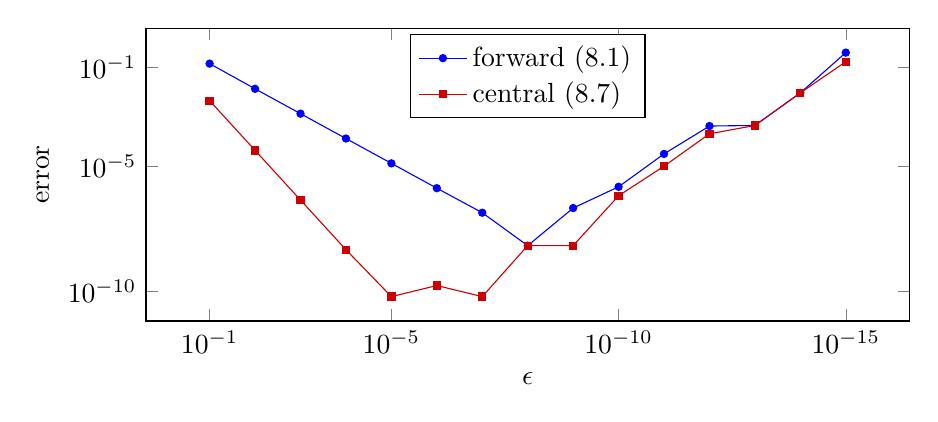
\begin{tikzpicture}
        \begin{loglogaxis}[width=.93\linewidth,height=5.3cm,
            xlabel={$\eps$},ylabel={error},x dir=reverse,
            xtick={1e-1,1e-5,1e-10,1e-15},
            ytick={1e-1,1e-5,1e-10},
            legend style={at={(0.5,0.98)},anchor=north},
            legend cell align=left]
          \addplot[blue,mark=*,mark size=1.3pt] coordinates {
            (1e-1,1.406e-01)(1e-2,1.364e-02)(1e-3,1.360e-03)(1e-4,1.359e-04)(1e-5,1.359e-05)
            (1e-6,1.359e-06)(1e-7,1.399e-07)(1e-8,6.603e-09)(1e-9,2.154e-07)(1e-10,1.548e-06)
            (1e-11,3.263e-05)(1e-12,4.323e-04)(1e-13,4.559e-04)(1e-14,9.338e-03)(1e-15,3.903e-01)};
          \addplot[red!80!black,mark=square*,mark size=1.3pt] coordinates {
            (1e-1,4.533e-03)(1e-2,4.530e-05)(1e-3,4.530e-07)(1e-4,4.531e-09)(1e-5,5.859e-11)
            (1e-6,1.635e-10)(1e-7,5.859e-11)(1e-8,6.603e-09)(1e-9,6.603e-09)(1e-10,6.727e-07)
            (1e-11,1.043e-05)(1e-12,2.103e-04)(1e-13,4.559e-04)(1e-14,9.338e-03)(1e-15,1.683e-01)};
          \legend{forward (8.1),central (8.7)}
        \end{loglogaxis}
      \end{tikzpicture}
    \end{column}
    \begin{column}{.42\textwidth}
      $f(x)=e^x$ at $x=1$, double precision. (Not in the book.)
      \begin{itemize}
        \item Right of the minimum: truncation, slope 1 and slope 2.
        \item Left of the minimum: cancellation, slope $-1$.
        \item Forward: best at $\eps\approx10^{-8}=\sqrt u$, error $7\times10^{-9}$.
        \item Central: best at $\eps\approx10^{-5}\approx u^{1/3}$, error $6\times10^{-11}$.
      \end{itemize}
    \end{column}
  \end{columns}
\end{frame}

\section{\S8.1 Finite differences: sparse Jacobians}

\begin{frame}{The Jacobian of a vector function}
  For $r:\R^n\to\R^m$,
  \begin{equation}
    J(x) = \left[\frac{\partial r_j}{\partial x_i}\right]_{\substack{j=1,\dots,m\\ i=1,\dots,n}}
    = \begin{bmatrix} \nabla r_1(x)^T\\ \vdots\\ \nabla r_m(x)^T \end{bmatrix}. \tag{8.9}
  \end{equation}
  If $J$ is Lipschitz with constant $L$, then
  $\|r(x+p)-r(x)-J(x)p\|\le (L/2)\|p\|^2$ (8.10), so
  \begin{equation}
    J(x)p\approx\frac{r(x+\eps p)-r(x)}{\eps}, \qquad
    \frac{\partial r}{\partial x_i}(x)\approx\frac{r(x+\eps e_i)-r(x)}{\eps}. \tag{8.11, 8.12}
  \end{equation}
  \begin{itemize}
    \item $J(x)p$: \alert{one extra evaluation}, accurate to $O(\eps)$ (inexact Newton, \S11.1).
    \item Full $J$ one column at a time: $n+1$ evaluations.
  \end{itemize}
\end{frame}

\begin{frame}{Example: a tridiagonal Jacobian}
  \begin{columns}[c]
    \begin{column}{.55\textwidth}
      \begin{equation}
        r(x) = \begin{bmatrix}
          2(x_2^3-x_1^2)\\
          3(x_2^3-x_1^2)+2(x_3^3-x_2^2)\\
          3(x_3^3-x_2^2)+2(x_4^3-x_3^2)\\
          \vdots\\
          3(x_n^3-x_{n-1}^2)
        \end{bmatrix} \tag{8.13}
      \end{equation}
    \end{column}
    \begin{column}{.42\textwidth}
      For $n=6$:
      \begin{equation}
        J = \begin{bmatrix}
          \times&\times&&&&\\
          \times&\times&\times&&&\\
          &\times&\times&\times&&\\
          &&\times&\times&\times&\\
          &&&\times&\times&\times\\
          &&&&\times&\times
        \end{bmatrix} \tag{8.14}
      \end{equation}
    \end{column}
  \end{columns}
  \vspace{1ex}
  Each $r_j$ depends on only two or three $x_i$. A perturbation of $x_1$ changes only $r_1, r_2$;
  re-evaluating $r_3,\dots,r_6$ for it is wasted work.
\end{frame}

\begin{frame}{Two columns from one evaluation}
  Perturb $x_1$ and $x_4$ together: $p=\eps(e_1+e_4)$. Columns 1 and 4 share no row, so
  \begin{equation}
    [r(x+p)]_{1,2} = [r(x+\eps e_1)]_{1,2}, \qquad
    [r(x+p)]_{3,4,5} = [r(x+\eps e_4)]_{3,4,5}. \tag{8.15}
  \end{equation}
  Hence (8.16)--(8.18):
  \[
    [J(x)e_1]_{1,2}\approx\frac{[r(x+p)-r(x)]_{1,2}}{\eps}, \qquad
    [J(x)e_4]_{3,4,5}\approx\frac{[r(x+p)-r(x)]_{3,4,5}}{\eps}.
  \]
  Likewise $p=\eps(e_2+e_5)$ and $p=\eps(e_3+e_6)$.
  \alert{Three extra evaluations of $r$ for every $n$}:
  \[
    p=\eps(e_1+e_4+e_7+\cdots),\quad p=\eps(e_2+e_5+e_8+\cdots),\quad p=\eps(e_3+e_6+e_9+\cdots).
  \]
  \readpp{pp.~197--200.}
\end{frame}

\begin{frame}{Graph coloring}
  \begin{columns}[c]
    \begin{column}{.62\textwidth}
      \textbf{Column intersection graph}: nodes $1,\dots,n$; an arc $i$--$k$ if some $r_j$ depends on both $x_i$ and $x_k$.

      \vspace{1ex}
      \textbf{Rule:} connected nodes get different colors. One perturbation per color:
      \[
        p=\eps(e_{i_1}+e_{i_2}+\cdots+e_{i_\ell}).
      \]
    \end{column}
    \begin{column}{.36\textwidth}
      \centering
      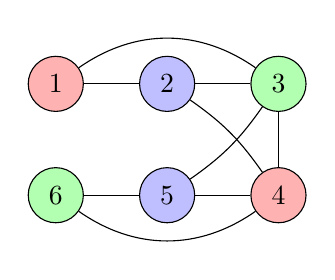
\begin{tikzpicture}[node distance=7mm,
          v/.style={circle,draw,minimum size=7mm,inner sep=0pt}]
        \node[v,fill=red!30] (1) {1};
        \node[v,fill=blue!25,right=of 1] (2) {2};
        \node[v,fill=green!30,right=of 2] (3) {3};
        \node[v,fill=red!30,below=of 3] (4) {4};
        \node[v,fill=blue!25,left=of 4] (5) {5};
        \node[v,fill=green!30,left=of 5] (6) {6};
        \draw (1)--(2)--(3)--(4)--(5)--(6);
        \draw (1) to[bend left=35] (3);
        \draw (2) to[bend left=10] (4);
        \draw (3) to[bend left=10] (5);
        \draw (4) to[bend left=35] (6);
      \end{tikzpicture}\\[1ex]
      Graph for (8.13), $n=6$; 3 colors (cf.\ Figure 8.1).
    \end{column}
  \end{columns}
  \begin{itemize}
    \item The minimum coloring is hard to find, but cheap heuristics do well
      (Curtis--Powell--Reid; Coleman--Mor\'e).
    \item Newsam--Ramsdell: at most $n_z$ extra evaluations, $n_z$ = max nonzeros per row of $J$.
  \end{itemize}
\end{frame}

\section{\S8.1 Finite differences: Hessians}

\begin{frame}{Approximating the Hessian}
  Apply the Jacobian techniques to $r=\nabla f$; symmetrize with $\tfrac12(A+A^T)$.

  \textbf{Hessian--vector product} (Newton--CG, Chapter 7):
  \begin{align}
    \nabla f(x+\eps p) &= \nabla f(x)+\eps\nabla^2 f(x)p+O(\eps^2), \tag{8.19}\\
    \nabla^2 f(x)p &\approx \frac{\nabla f(x+\eps p)-\nabla f(x)}{\eps}. \tag{8.20}
  \end{align}
  One gradient evaluation, error $O(\eps)$. Same as (7.10).

  \textbf{Function values only} (from (8.8) with $p=\eps e_i,\ \eps e_j,\ \eps(e_i+e_j)$):
  \begin{equation}
    \frac{\partial^2 f}{\partial x_i\partial x_j}(x) =
    \frac{f(x+\eps e_i+\eps e_j)-f(x+\eps e_i)-f(x+\eps e_j)+f(x)}{\eps^2}+O(\eps). \tag{8.21}
  \end{equation}
  Full Hessian: $n(n+1)/2+n$ extra points.
\end{frame}

\begin{frame}{Sparse Hessians: the arrowhead example}
  \begin{columns}[c]
    \begin{column}{.47\textwidth}
      \begin{equation}
        f(x) = x_1\sum_{i=1}^n i^2x_i^2. \tag{8.22}
      \end{equation}
      Row 1 is full, so in the intersection graph for $\nabla f$ every node is connected to every other.
      Coloring needs $n$ colors: \alert{$n$ extra gradients.}
    \end{column}
    \begin{column}{.51\textwidth}
      For $n=6$:
      \begin{equation}
        \nabla^2 f = \begin{bmatrix}
          \times&\times&\times&\times&\times&\times\\
          \times&\times&&&&\\
          \times&&\times&&&\\
          \times&&&\times&&\\
          \times&&&&\times&\\
          \times&&&&&\times
        \end{bmatrix} \tag{8.23}
      \end{equation}
    \end{column}
  \end{columns}
\end{frame}

\begin{frame}{Exploiting symmetry}
  \begin{enumerate}
    \item $p=\eps e_1$ gives column 1, hence row 1 too, by symmetry.
    \item Only the diagonal entries $2,\dots,6$ remain. They do not interfere:
      \begin{equation}
        p = \eps(e_2+e_3+\cdots+e_6) = \eps(0,1,1,1,1,1)^T, \tag{8.24}
      \end{equation}
      \[
        \frac{\partial^2 f}{\partial x_i^2}(x)\approx\frac{\nabla f(x+p)_i-\nabla f(x)_i}{\eps},\qquad i=2,\dots,6.
      \]
  \end{enumerate}
  \alert{Whole Hessian from $\nabla f$ at $x$ and two other points}, for any $n$.

  \begin{block}{Coloring rule for symmetric Hessians (Coleman--Mor\'e)}
    Use the \textbf{adjacency graph} (arc $i$--$k$ if $i\neq k$ and $\partial^2 f/\partial x_i\partial x_k\neq0$).
    Adjacent nodes get different colors, \emph{and} every path of length 3 uses at least 3 colors.
  \end{block}
  \readpp{pp.~201--204.}
\end{frame}

\section{\S8.2 Automatic differentiation: the forward mode}

\begin{frame}{Automatic differentiation}
  \begin{itemize}
    \item Any function, however complicated, is evaluated as a sequence of
      \textbf{elementary operations} with one or two arguments: $+,-,\times,/,a^b$, $\sin$, $\exp$, $\log$, \dots
    \item Apply the chain rule to each operation. For $h(y(x))$ with $y\in\R^m$:
      \begin{equation}
        \nabla_x h(y(x)) = \sum_{i=1}^m \frac{\partial h}{\partial y_i}\nabla y_i(x). \tag{8.25}
      \end{equation}
    \item The tool does the bookkeeping: source transformation (ADIFOR) or recording the computation at run time (ADOL-C).
  \end{itemize}
  The results are \alert{exact derivatives of the program}, up to roundoff. No $\eps$, no truncation error.

  Two basic modes: \textbf{forward} and \textbf{reverse}.
\end{frame}

\begin{frame}{An example and its computational graph}
  \begin{columns}[c]
    \begin{column}{.47\textwidth}
      \begin{equation}
        f(x) = (x_1x_2\sin x_3+e^{x_1x_2})/x_3 \tag{8.26}
      \end{equation}
      \vspace{-3ex}
      \begin{equation}
        \begin{aligned}
          x_4&=x_1x_2, & x_5&=\sin x_3,\\
          x_6&=e^{x_4}, & x_7&=x_4x_5,\\
          x_8&=x_6+x_7, & x_9&=x_8/x_3.
        \end{aligned} \tag{8.27}
      \end{equation}
    \end{column}
    \begin{column}{.51\textwidth}
      \centering
      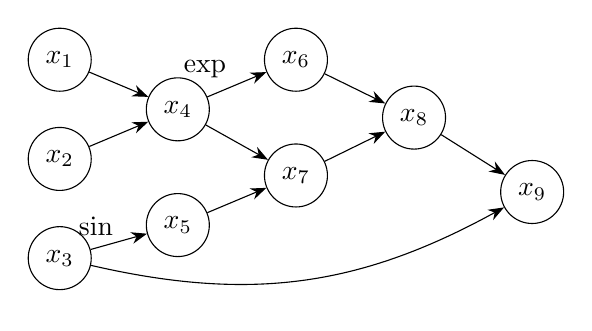
\begin{tikzpicture}[>={Stealth[length=2mm]},xscale=1.0,yscale=1.05,
          v/.style={circle,draw,minimum size=8mm,inner sep=0pt}]
        \node[v] (x1) at (0,2.4) {$x_1$};
        \node[v] (x2) at (0,1.2) {$x_2$};
        \node[v] (x3) at (0,0) {$x_3$};
        \node[v] (x4) at (1.5,1.8) {$x_4$};
        \node[v] (x5) at (1.5,0.4) {$x_5$};
        \node[v] (x6) at (3,2.4) {$x_6$};
        \node[v] (x7) at (3,1.0) {$x_7$};
        \node[v] (x8) at (4.5,1.7) {$x_8$};
        \node[v] (x9) at (6,0.8) {$x_9$};
        \draw[->] (x1)--(x4); \draw[->] (x2)--(x4);
        \draw[->] (x3)--node[above left=-2pt,pos=.5]{$\sin$}(x5);
        \draw[->] (x4)--node[above left=-1pt,pos=.45]{$\exp$}(x6);
        \draw[->] (x4)--(x7); \draw[->] (x5)--(x7);
        \draw[->] (x6)--(x8); \draw[->] (x7)--(x8);
        \draw[->] (x8)--(x9); \draw[->] (x3) to[bend right=20] (x9);
      \end{tikzpicture}\\[.5ex]
      Computational graph (cf.\ Figure 8.2)
    \end{column}
  \end{columns}
  \vspace{1ex}
  Node $i$ is a \textbf{parent} of node $j$ if there is an arc $i\to j$.
  A node can be evaluated once all its parents are known: the \textbf{forward sweep}.
  The tool builds this graph itself; the user does not write (8.27).
\end{frame}

\begin{frame}{The forward mode}
  Fix a \textbf{seed vector} $p\in\R^n$. Carry, alongside each $x_i$, its directional derivative
  \begin{equation}
    D_px_i \overset{\text{def}}{=} (\nabla x_i)^Tp = \sum_{j=1}^3\frac{\partial x_i}{\partial x_j}p_j,
    \qquad i=1,\dots,9. \tag{8.28}
  \end{equation}
  Start: $D_px_i=p_i$ for the independent variables. At each node, by the chain rule,
  \begin{equation}
    x_7=x_4x_5:\qquad D_px_7 = x_5\,D_px_4 + x_4\,D_px_5. \tag{8.29}
  \end{equation}
  At the end: $D_px_9 = \nabla f(x)^Tp$. \alert{One sweep, one directional derivative.}

  \begin{itemize}
    \item The values $x_i, D_px_i$ can be overwritten once all children of node $i$ are done.
  \end{itemize}
\end{frame}

\begin{frame}{Forward mode at $x=(1,2,\pi/2)^T$ with seed $p=e_1$}
  \centering
  \renewcommand{\arraystretch}{1.15}
  \begin{tabular}{llll}
    \toprule
    node & value $x_i$ & rule & $D_{e_1}x_i$\\
    \midrule
    $x_1,x_2,x_3$ & $1,\ 2,\ \pi/2$ & seed & $1,\ 0,\ 0$\\
    $x_4=x_1x_2$ & $2$ & $x_2D x_1+x_1Dx_2$ & $2$\\
    $x_5=\sin x_3$ & $1$ & $\cos x_3\,Dx_3$ & $0$\\
    $x_6=e^{x_4}$ & $e^2$ & $e^{x_4}Dx_4$ & $2e^2$\\
    $x_7=x_4x_5$ & $2$ & $x_5Dx_4+x_4Dx_5$ & $2$\\
    $x_8=x_6+x_7$ & $2+e^2$ & $Dx_6+Dx_7$ & $2+2e^2$\\
    $x_9=x_8/x_3$ & $(4+2e^2)/\pi$ & $Dx_8/x_3-x_8Dx_3/x_3^2$ & $(4+4e^2)/\pi$\\
    \bottomrule
  \end{tabular}

  \vspace{1.5ex}
  \raggedright
  So $\partial f/\partial x_1 = (4+4e^2)/\pi$. For $\partial f/\partial x_2$ and $\partial f/\partial x_3$:
  two more sweeps, with $p=e_2$ and $p=e_3$. (Exercise 8.7.)
\end{frame}

\begin{frame}{Cost and implementation of the forward mode}
  Division $z\leftarrow w/y$ becomes
  \begin{equation}
    D_pz \leftarrow \frac1y D_pw - \frac{w}{y^2}D_py. \tag{8.30}
  \end{equation}
  \begin{itemize}
    \item Full gradient: seeds $p=e_1,\dots,e_n$ carried together.
      One division in $f$ costs about $2n$ multiplications and $n$ additions:
      \alert{work and storage grow by up to a factor $n$.}
    \item Sparse storage helps: many $D_{e_j}x_i$ are zero early in the graph.
    \item Implementation: a \textbf{precompiler} that writes the extended code, or
      \textbf{operator overloading} (C++), which extends the data types transparently.
  \end{itemize}
  \readpp{pp.~204--207.}
\end{frame}

\section{\S8.2 Automatic differentiation: the reverse mode}

\begin{frame}{The reverse mode}
  First the forward sweep computes $f$, and stores every $x_i$ and every arc partial $\partial x_j/\partial x_i$.
  Then a \textbf{reverse sweep} goes from the output back to the inputs.

  Each node has an \textbf{adjoint} $\xb_i$; start with $\xb_i=0$, except $\xb_N=1$ at the output.
  \begin{block}{Reverse sweep}
    \vspace{-1ex}
    \begin{equation}
      \frac{\partial f}{\partial x_i} = \sum_{j\text{ a child of }i}\frac{\partial f}{\partial x_j}\frac{\partial x_j}{\partial x_i},
      \qquad
      \xb_i \mathrel{+}= \frac{\partial f}{\partial x_j}\frac{\partial x_j}{\partial x_i}. \tag{8.31, 8.32}
    \end{equation}
  \end{block}
  When all children of $i$ have contributed, $\xb_i=\partial f/\partial x_i$: node $i$ is \textbf{finalized}
  and passes its contribution on to its parents.

  The sweep works with \alert{numbers, not formulas.}
\end{frame}

\begin{frame}{Reverse mode at $x=(1,2,\pi/2)^T$: the arc partials}
  \centering
  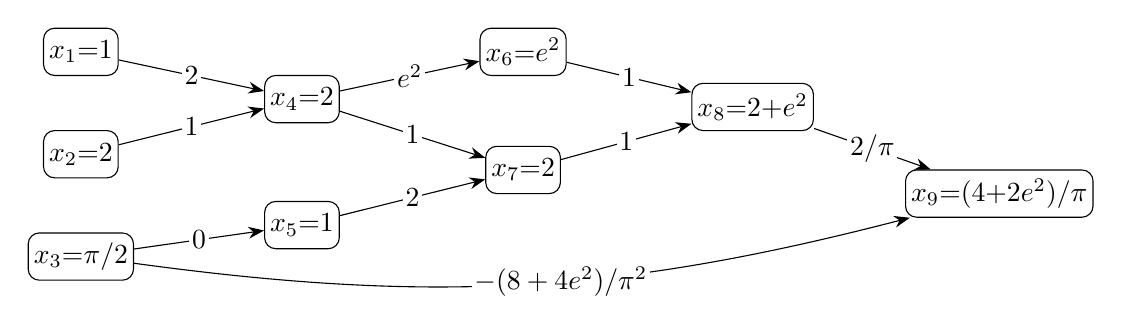
\begin{tikzpicture}[>={Stealth[length=2mm]},
      v/.style={rectangle,rounded corners,draw,minimum height=6mm,inner sep=2pt},
      a/.style={fill=white,inner sep=1pt},xscale=1.08]
    \node[v] (x1) at (0,2.6) {$x_1{=}1$};
    \node[v] (x2) at (0,1.3) {$x_2{=}2$};
    \node[v] (x3) at (0,0) {$x_3{=}\pi/2$};
    \node[v] (x4) at (2.6,2.0) {$x_4{=}2$};
    \node[v] (x5) at (2.6,0.4) {$x_5{=}1$};
    \node[v] (x6) at (5.2,2.6) {$x_6{=}e^2$};
    \node[v] (x7) at (5.2,1.1) {$x_7{=}2$};
    \node[v] (x8) at (7.9,1.9) {$x_8{=}2{+}e^2$};
    \node[v] (x9) at (10.8,0.8) {$x_9{=}(4{+}2e^2)/\pi$};
    \draw[->] (x1)--node[a]{2}(x4);
    \draw[->] (x2)--node[a]{1}(x4);
    \draw[->] (x3)--node[a]{0}(x5);
    \draw[->] (x4)--node[a]{$e^2$}(x6);
    \draw[->] (x4)--node[a]{1}(x7);
    \draw[->] (x5)--node[a]{2}(x7);
    \draw[->] (x6)--node[a]{1}(x8);
    \draw[->] (x7)--node[a]{1}(x8);
    \draw[->] (x8)--node[a]{$2/\pi$}(x9);
    \draw[->] (x3) to[bend right=12] node[a,pos=.55]{$-(8+4e^2)/\pi^2$}(x9);
  \end{tikzpicture}

  \vspace{1ex}
  \raggedright
  Arc labels: $\partial x_j/\partial x_i$, computed and stored during the forward sweep (cf.\ Figure 8.3).
  Example: $x_9=x_8/x_3$ gives $\partial x_9/\partial x_3 = -x_8/x_3^2 = -(8+4e^2)/\pi^2$.
\end{frame}

\begin{frame}{Reverse mode at $x=(1,2,\pi/2)^T$: the sweep}
  Start with $\xb_9=1$; node 9 is finalized. Its parents are nodes 3 and 8:
  \begin{equation}
    \xb_3 \mathrel{+}= 1\cdot\frac{-(2+e^2)}{(\pi/2)^2} = \frac{-8-4e^2}{\pi^2}, \qquad
    \xb_8 \mathrel{+}= 1\cdot\frac{1}{\pi/2} = \frac2\pi. \tag{8.33}
  \end{equation}
  Node 3 still waits for node 5. Node 8 is finalized, and so on down the graph:
  \[
    \begin{aligned}
      &\xb_6=\xb_7=\tfrac2\pi, \qquad
       \xb_4 = \tfrac2\pi e^2+\tfrac2\pi\cdot1 = \tfrac{2+2e^2}{\pi}, \qquad
       \xb_5 = \tfrac2\pi\cdot2=\tfrac4\pi,\\
      &\xb_3 \mathrel{+}= \tfrac4\pi\cdot0, \qquad
       \xb_1 = \xb_4\cdot2, \qquad \xb_2=\xb_4\cdot1.
    \end{aligned}
  \]
  \begin{block}{Result: one reverse sweep gives the whole gradient}
    \vspace{-1ex}
    \[
      \nabla f(x) = (\xb_1,\xb_2,\xb_3) = \Bigl(\tfrac{4+4e^2}{\pi},\ \tfrac{2+2e^2}{\pi},\ \tfrac{-8-4e^2}{\pi^2}\Bigr).
    \]
  \end{block}
\end{frame}

\begin{frame}{The cheap gradient, and its price}
  \begin{block}{Cost of the reverse mode for $f:\R^n\to\R$}
    The gradient costs \alert{at most 4--5 times} the arithmetic of $f$ alone, \alert{independent of $n$}.
  \end{block}
  Example (8.33): two multiplications, a division and two additions,
  against one division in the forward sweep.
  The forward mode needs up to $n$ times the work of $f$.

  \textbf{The price is memory.} The whole graph must be stored for the reverse sweep.
  At 20 bytes per node, one second of a 100 Mflop computation can need 2 GB.
  \begin{itemize}
    \item \textbf{Checkpointing}: store only some states; recompute the pieces in between during the reverse sweep.
      This trades extra arithmetic for less storage.
  \end{itemize}
  \readpp{pp.~207--210.}
\end{frame}

\section{\S8.2 Automatic differentiation: vector functions}

\begin{frame}{Vector functions and partial separability}
  For $r:\R^n\to\R^m$ the graph has $m$ output nodes.
  \textbf{Partially separable} $f$ (Chapter 7):
  \begin{equation}
    f(x) = \sum_{i=1}^{ne}f_i(x),\qquad
    r(x) = \begin{bmatrix} f_1(x)\\ \vdots\\ f_{ne}(x)\end{bmatrix},\qquad
    \nabla f(x) = J(x)^Te, \tag{8.34, 8.35}
  \end{equation}
  with $e=(1,\dots,1)^T$. Each $f_i$ depends on a few $x_j$: $J$ is sparse, and coloring makes it cheap.
  \begin{itemize}
    \item Gay: automatic detection of the partially separable structure.
    \item Constrained problems: evaluate $f$ and all $c_j$ together as one vector function;
      shared subexpressions (like $x_4$ in (8.27)) are computed once.
  \end{itemize}
\end{frame}

\begin{frame}{Jacobians: $Jp$ by forward mode, $J^Tq$ by reverse mode}
  \begin{columns}[T]
    \begin{column}{.48\textwidth}
      \begin{block}{Forward, seed $p\in\R^n$}
        One sweep gives $J(x)p$.\\
        Full $J$: $n$ seeds, or fewer with coloring of columns.\\
        Cost $\approx$ number of seeds $\times$ cost of $r$.
      \end{block}
    \end{column}
    \begin{column}{.48\textwidth}
      \begin{block}{Reverse, seed $q\in\R^m$}
        One sweep on $r(x)^Tq$ gives
        $\nabla[r(x)^Tq] = J(x)^Tq$.\\
        Full $J$: $m$ seeds, or coloring of $J^T$.\\
        Cost $\le 5\times$ number of seeds $\times$ cost of $r$.
      \end{block}
    \end{column}
  \end{columns}
  \vspace{1ex}
  \begin{itemize}
    \item $m\ll n$: reverse. $m\gg n$: forward. The two can be combined (some columns by forward, the remaining rows by reverse).
    \item Inexact Newton (\S11.1) needs only $J(x)p$: \alert{one forward sweep}, about the cost of $r$.
  \end{itemize}
  \readpp{pp.~210--213.}
\end{frame}

\section{\S8.2 Automatic differentiation: Hessians}

\begin{frame}{Hessians by the forward mode}
  For two seeds $p,q$, carry also
  \begin{equation}
    D_{pq}x_i = p^T(\nabla^2x_i)\,q, \qquad D_{pq}x_i=0 \text{ at the inputs}. \tag{8.36}
  \end{equation}
  Propagation rules, from the chain rule:
  \begin{align}
    x_i=x_j+x_k:&\quad D_px_i=D_px_j+D_px_k,\quad D_{pq}x_i=D_{pq}x_j+D_{pq}x_k, \tag{8.37}\\
    x_i=L(x_j):&\quad D_px_i=L'(x_j)D_px_j, \tag{8.38b}\\
    &\quad D_{pq}x_i=L''(x_j)(D_px_j)(D_qx_j)+L'(x_j)D_{pq}x_j. \tag{8.38c}
  \end{align}
  At the output: $D_{pq}f = p^T\nabla^2 f(x)\,q$.
  Note that (8.38c) needs both $D_p$ and $D_q$.
\end{frame}

\begin{frame}{Cost of forward-mode Hessians}
  \begin{itemize}
    \item \textbf{Full Hessian}: pairs $(e_j,e_k)$, $k\le j$, only where $[\nabla^2 f]_{jk}$ may be nonzero.
      Work: a small multiple of $1+n+N_z(\nabla^2 f)$ times the cost of $f$.
    \item \textbf{Hessian--vector product} $\nabla^2 f(x)q$: carry $D_{e_j}x_i$, $D_qx_i$, $D_{e_jq}x_i$.
      The output holds $e_j^T\nabla^2f(x)q=[\nabla^2 f(x)q]_j$.
      Work: a small multiple of $2n$.
  \end{itemize}
  \textbf{Univariate trick.} Avoid the cross terms $D_{pq}$, $p\neq q$:
  \begin{equation}
    [\nabla^2 f]_{ij} = \tfrac12\bigl[(e_i+e_j)^T\nabla^2 f(e_i+e_j) - e_i^T\nabla^2 f e_i - e_j^T\nabla^2 f e_j\bigr]. \tag{8.39}
  \end{equation}
  With $\psi(t)=f(x+tp)$ (8.40): $D_pf=\psi'(0)$ and $D_{pp}f=\psi''(0)$. This extends to higher derivatives.
\end{frame}

\begin{frame}{Hessians by the reverse mode}
  \begin{block}{Hessian--vector product: reverse over forward}
    \begin{enumerate}
      \item Forward sweep: compute $f$ and $\nabla f(x)^Tq$ (carry $x_i$ and $D_qx_i$).
      \item Reverse sweep on the scalar $\nabla f(x)^Tq$:
        \[
          \frac{\partial}{\partial x_i}\bigl(\nabla f(x)^Tq\bigr) = [\nabla^2 f(x)q]_i,\qquad i=1,\dots,n.
        \]
    \end{enumerate}
  \end{block}
  \begin{itemize}
    \item Cost: about \alert{12 times} the cost of $f$, \alert{independent of $n$}.
    \item Full Hessian: $q=e_1,\dots,e_n$, up to $12n$. Sparse with known structure: $12N_c$, where $N_c$ is the number of seed vectors from coloring.
  \end{itemize}
  \readpp{pp.~213--216.}
\end{frame}

\begin{frame}{Current limitations}
  \begin{itemize}
    \item \textbf{AD differentiates the program, not the mathematics.}
      If $f$ needs a PDE solve, the computed value is $\hat f(x)=f(x)+\tau(x)$.
      The truncation error $|\tau|$ is small, but $\tau'$ need not be, so $\hat f'$ can be far from $f'$.
      Finite differences have the same problem.
    \item \textbf{Branches.} The linear function $f(x)=x-1$, coded as
      \[
        \texttt{if (x == 1.0) then f = 0.0 else f = x - 1.0}
      \]
      gives $f'(1)=0$ by AD.
  \end{itemize}
  \begin{block}{The book's conclusion}
    AD is a powerful set of tools, but not a panacea: the user is still responsible for thinking about derivative calculations.
  \end{block}
  \readpp{pp.~216--217.}
\end{frame}

\begin{frame}{AD today (not in the book)}
  \begin{itemize}
    \item The reverse mode is \textbf{backpropagation}. Training a network with millions of parameters
      is feasible because the gradient costs a small constant times the loss, independent of $n$.
    \item JAX and PyTorch expose both modes:
      \texttt{jvp} = forward mode ($J p$), \texttt{vjp} = reverse mode ($J^T q$).
      \texttt{jax.hessian} uses forward over reverse.
    \item Checkpointing is ``gradient checkpointing'' in deep learning: the same memory--compute trade-off.
  \end{itemize}
\end{frame}

\section{Chapter 8: summary}

\begin{frame}{Chapter 8 in one table}
  \centering
  \renewcommand{\arraystretch}{1.1}
  \begin{tabular}{lll}
    \toprule
    Quantity & Method & Cost (in units of $f$ or $r$)\\
    \midrule
    $\nabla f$, error $\sqrt u$ & forward difference (8.1) & $n+1$\\
    $\nabla f$, error $u^{2/3}$ & central difference (8.7) & $2n+1$\\
    $\nabla f$, exact & forward mode & $\sim n$\\
    $\nabla f$, exact & reverse mode & $\le 5$\\
    $J(x)p$ & FD (8.11) or forward mode & $1$\\
    sparse $J$ & FD or AD with coloring & number of colors\\
    $\nabla^2 f\,q$ & FD of gradient (8.20) & 1 gradient\\
    $\nabla^2 f\,q$ & reverse over forward & $\sim 12$\\
    \bottomrule
  \end{tabular}
\end{frame}

\begin{frame}{Three results to carry forward}
  \begin{enumerate}
    \item \textbf{Finite differences trade truncation against cancellation.}
      Forward: $\eps=\sqrt u$, about half the digits. Central: $\eps=u^{1/3}$, about two thirds.
    \item \textbf{Sparsity makes differencing cheap.}
      Columns that share no row are perturbed together; graph coloring picks the groups.
      Symmetry reduces the count further for Hessians.
    \item \textbf{The reverse mode gives the gradient at a constant cost.}
      At most about 5 times the cost of $f$, for any $n$, paid for in memory.
  \end{enumerate}
  \vspace{1ex}
  Worked through: (8.26) in both modes, the arrowhead Hessian (8.22).
\end{frame}

\begin{frame}{Homework {\normalsize (problems 5--6 are not in the book)}}
  \begin{enumerate}
    \item Exercise 8.1: for the central difference, $\eps\approx u^{1/3}$ and error $\approx u^{2/3}$.
    \item Exercise 8.5: adjacency graph of (8.22); show that the two-color scheme is valid.
    \item Exercise 8.9: finish the reverse sweep for (8.26) at $x=(1,2,\pi/2)^T$; give the order in which nodes are finalized.
    \item Exercise 8.10: reverse-sweep operations for $x_k\leftarrow x_ix_j$ and $x_k\leftarrow\cos x_i$.
    \item Reproduce the V-shaped plot for $f(x)=\sin x$ at $x=1$, $\eps=10^{-1},\dots,10^{-15}$.
      Mark $\sqrt u$ and $u^{1/3}$.
    \item Write a gradient checker: compare your analytic (or AD) gradient of Rosenbrock's function (2.22)
      with central differences, and report the largest relative error.
  \end{enumerate}
\end{frame}

\end{document}
